\subsection{Matter-regime fields as retained transport behavior}
\label{man:matter-regime-fields}

Matter-regime rows are recorded here as windowed behavior of retained ominion transport. This layer is a classification scaffold: the rows below are exact integer/rational signatures for regimes, while regime-specific predictions require their own declared source chains, scripts, and tests.

\RetentionBlock
{matter-regime retained transport field family}
{duon/tetron transport behavior by regime class}
{external sector and material benchmark layers}
{regime-specific exact row with declared source chain and tests}
{classification window only}
{pending until regime-specific script/test support exists}

\begin{table}[H]
\centering
\caption{Matter-regime classification scaffold.}
\label{tab:matter-regime-scaffold}
\begin{threeparttable}
\small
\begin{tabularx}{\linewidth}{@{}lXX@{}}
\toprule
Regime & Retained field & Dominant exact variables \\
\midrule
Gas & sparse mobile duon/tetron faces & collision window, integer step ratios, weak shell persistence \\
Plasma & polarized mobile boundary field & \((Q,S)\), \(\chi\), phase-cycle residues, export/reclosure \\
Liquid & dense near-neutral reclosure field & burden flow, torsion ratios, phase lag \\
Solid & constrained ominion / lattice-like chain & fixed adjacency, stress channels, transport ratios \\
Wire current & conductive transport subfield inside solid host & \(u^{(\mathrm{tr})}\), \((Q,S)\), \(w_\perp\), sheath boundary \\
Ring fields & shell-selected transport field & occupancy bands, gaps, long-window phase locking \\
\bottomrule
\end{tabularx}
\ManualTableNote{This table is a scaffold. Validated applications require exact rows and tests.}
\end{threeparttable}
\end{table}

\begin{table}[H]
\centering
\caption{Matter-regime exact scaffold signatures.}
\label{tab:matter-regime-exact-scaffold-signatures}
\begin{threeparttable}
\small
\begin{tabularx}{\linewidth}{@{}lccccX@{}}
\toprule
Regime & \(Q/S\) & Torsion & Persistence & Balance & Status \\
\midrule
Gas & \(1/9\) & \(1/1\) & \(1/5\) & \(11/144\) & scaffold \\
Plasma & \(5/12\) & \(3/2\) & \(2/7\) & \(4/36\) & scaffold \\
Liquid & \(0\) & \(5/4\) & \(3/4\) & \(-1/144\) & scaffold \\
Solid & \(0\) & \(7/4\) & \(6/7\) & \(-11/144\) & scaffold \\
Wire current & \(3/11\) & \(2/1\) & \(5/6\) & \(1/144\) & worked in Section~\ref{man:transport-current-fields} \\
Ring fields & \(2/13\) & \(4/3\) & \(8/9\) & \(-1/24\) & scaffold \\
\bottomrule
\end{tabularx}
\ManualTableNote{The balance column is the exact row \((\mathrm{mobility}-\mathrm{reclosure})/|\omega|_{\mathrm{bip}_0}\) from the manual-local scaffold setup.}
\end{threeparttable}
\end{table}

\begin{figure}[H]
\centering
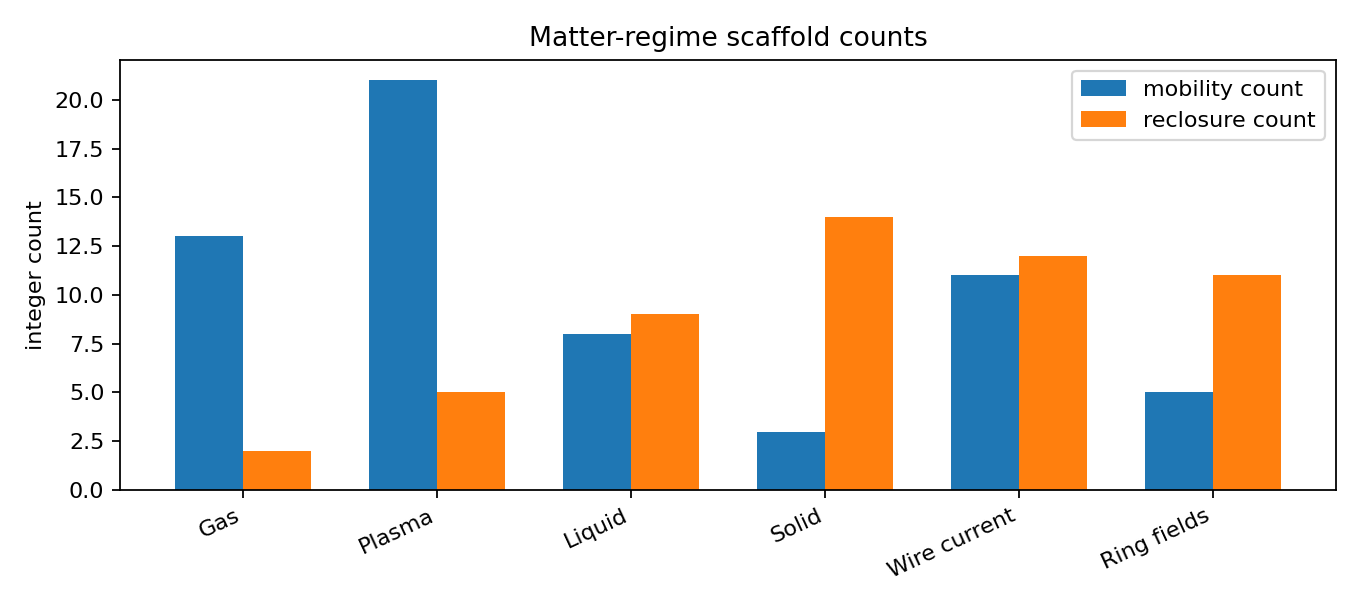
\includegraphics[width=0.86\linewidth]{figures/matter/01_matter_transport_scaffold.png}
\caption{Matter-regime scaffold counts generated from exact rows.}
\label{fig:matter-transport-scaffold}
\end{figure}

\paragraph{Reproducibility.}
The raw setup, script, derived CSV, figure, and tests are manual-local. They are listed in the manual artifact map and audited by the manual-local application-scaffold audit.
